% HMC Math dept HW template example
% v0.04 by Eric J. Malm, 10 Mar 2005
\documentclass[12pt,letterpaper,boxed]{hmcpset}
\usepackage[francais]{babel}
\usepackage[utf8x]{inputenc}
\usepackage[T1]{fontenc}
\usepackage{enumitem}
% set 1-inch margins in the document
\usepackage[margin=1in]{geometry}

\usepackage{empheq}




\newcommand*\widefbox[1]{\fbox{\hspace{2em}#1\hspace{2em}}}
% include this if you want to import graphics files with /includegraphics
\usepackage{graphicx}

\newcommand{\property}{\mathbf{P}}


% info for header block in upper right hand corner
\name{Tristan Stérin}
\class{FDI}
\assignment{DM \#2}
\duedate{21/12/2015}

\usepackage[dvipsnames,svgnames]{xcolor}  
\usepackage{tikz}
\usetikzlibrary{%
  shapes,
  decorations.shapes,
  decorations.fractals,
  decorations.markings,
  shadows
}

\newsavebox{\mycandle}
\savebox{\mycandle}{ 
\begin{tikzpicture}[scale=.1]
\shade[top color=yellow,bottom color=red] (0,0) .. controls (1,.2) and (1,.5) .. (0,2) .. controls (-1,.5)  and  (-1,.2) .. (0,0);
\fill[yellow!90!black] (.8,0) rectangle (-.8,-5); 
\end{tikzpicture} } 

\tikzset{
  paint/.style={draw=#1!50!black, fill=#1!50},
  my star/.style={decorate,decoration={shape backgrounds,shape=star},
                  star points=#1}
}  


\begin{document}

\problemlist{Exercice 1}

\begin{problem}[Question 1]
Montrer que les fonctions suivantes sont primitves récursives.
\begin{itemize}
  \item[(\textit{a})] Les fonctions constantes $c_{a}(n)=a$.
  \item[(\textit{b})] La fonction \textit{somme} définie par $somme(n,m) = n+m$.
  \item[(\textit{c})] La fonction \textit{prédécesseur} p définie par $p(n) = max(0,n-1)$.
  \item[(\textit{d})] La fonction \textit{prod} définie par $prod(n,m) = nm$.
  \item[(\textit{e})] La fonction \textit{eq0} définie par $eq0(m) = 1$ si $m = 0$ et $eq0(m) = 0$ sinon.
  \item[(\textit{f})]  La fonction \textit{eq} définie par $eq(n,m) = 1$ si $m = n$ et $eq(n,m) = 0$ sinon.
  \item[(\textit{g})] Toute fonction $f : N \to \mathbb{N}$ à support fini : $$\exists E \subseteq \mathbb{N}, \, |E| < \infty \quad x \notin E \implies f(x) = 0$$.
\end{itemize}


\end{problem}

\begin{solution}[(a)]
Soit $a \in \mathbb{N}$.\\ On montre que : 
$$  \boxed{\forall n \in \mathbb{N}, \, c_{a}(n) = s^{a}(\odot(n))} $$ 
\\

\noindent Avec $s^{a}$ $s$ composé $a$ fois. \\
Une récurrence sur $a$ montre que $s^a(0) = a$. \\
Écrit sous cette forme on constate que $c_{a}$ est récursive primitive par $a+1$ applications du schéma de composition. \\


%\begin{align*}
 %\limsup_{n \to \infty} \, (a_n + b_n)
 % &= \lim_{n \to \infty} C_n \\
  %&\leq \lim_{n \to \infty} \, (A_n + B_n)
  %= \lim_{n \to \infty} A_n + \lim_{n \to \infty} B_n
  %= \limsup_{n \to \infty} a_n + \limsup_{n \to \infty} b_n.
%\end{align*}
\end{solution}

\begin{solution}[(b)]
On définit \textit{somme'} : 

\ \\
\begin{empheq}[box=\widefbox]{align*}
  \forall (n,m) \in \mathbb{N}^{2}, \quad & somme'(n,0) = n \\ 
  & somme'(n,m+1) = (s \circ p^{3}_{3})(n,m,somme'(n,m))
\end{empheq}
\ \\

\noindent$somme'$ est PR par application une fois du schéma de récurrence primitive : $s \circ p^{3}_{3}$ est PR par composition. 
\newpage
\noindent Soit $n \in \mathbb{N}$, on montre par récurrence sur $m\in\mathbb{N}$ :
$$ \property(m) \, : \, \text{"}somme'(n,m) = somme(n,m) = n+m\text{"}$$

\begin{itemize}
\item 
$\property(0)$ : $somme'(n,0) = n = n + 0$

\item \textbf{Hérédité} : 
Soit $m \in \mathbb{N}$ tel que $\property(m)$, on a :
\begin{align*} somme'(n,m+1) & = (s \circ p^{3}_{3})(n,m,somme'(n,m)) \\
					      & = s(somme'(n,m)) \\
					      & = s(n+m) \\
					      & = (n + m) + 1 \\
					      & = n + (m+1) \\
					     \end{align*}
D'où $\property(m+1)$. 
\end{itemize}
\ \\
Donc $somme = somme'$ et $somme$ est PR.



%\begin{align*}
 %\limsup_{n \to \infty} \, (a_n + b_n)
 % &= \lim_{n \to \infty} C_n \\
  %&\leq \lim_{n \to \infty} \, (A_n + B_n)
  %= \lim_{n \to \infty} A_n + \lim_{n \to \infty} B_n
  %= \limsup_{n \to \infty} a_n + \limsup_{n \to \infty} b_n.
%\end{align*}
\end{solution}

\begin{solution}[(c)]
L'énoncé est un peu ambigü comme soulevé dans la FAQ. \\
On considère malgré les définitions que les $\mathbb{N}^0 \to \mathbb{N}$ sont PR 
(les constantes sont PR, ça justifie). \\
Ainsi on peut définir des fonctions à une seule variable en schéma de récursion primitive. \\
On montre que p vérifie :
\ \\
\begin{empheq}[box=\widefbox]{align*}
    & p(0) = 0 \\ 
  \forall n \in \mathbb{N}, \quad & p(n+1) =  p^{2}_{1}(n,p(n))
\end{empheq}
\ \\

En effet, $p(0) = max(0,-1) = 0$ et pour $n \in \mathbb{N}$ : $$p(n+1) = max(0,n) = n = p^{2}_{1}(n,p(n))$$
Sous cette forme on constate que $p$ est PR.


\end{solution}


\begin{solution}[(d)]

On définit \textit{prod'} : 

\ \\
\begin{empheq}[box=\widefbox]{align*}
  \forall (n,m) \in \mathbb{N}^{2}, \quad & prod'(n,0) = 0 \\ 
  & prod'(n,m+1) = somme_{13}(n,m,prod'(n,m)) \\
  \text{avec : }&somme_{13}(x_{1},x_{2},x_{3}) = somme(p^{3}_{1}(x_{1},x_{2},x_{3}),p^{3}_{3}(x_{1},x_{2},x_{3}))
\end{empheq}
\ \\

\noindent$somme_{13}$ est PR par schéma de composition et 1b) donc $prod'$ est PR par schéma de récurrence.
\newpage
 \noindent Soit $n \in \mathbb{N}$, on montre par récurrence sur $m\in\mathbb{N}$ :
$$ \property(m) \, : \, \text{"}prod'(n,m) = prod(n,m) = n*m\text{"}$$

\begin{itemize}
\item 
$\property(0)$ : $prod'(n,0) = 0 = n*0$

\item \textbf{Hérédité} : 
Soit $m \in \mathbb{N}$ tel que $\property(m)$, on a :
\begin{align*} prod'(n,m+1) & = somme_{13}(n,m,prod'(n,m)) \\
					      & = n+prod'(n,m) \\
					      & = n+n*m \\
					      & = n*(m+1) \\
					     \end{align*}
D'où $\property(m+1)$. 
\end{itemize}
\ \\
Donc $prod = prod'$ et $prod$ est PR.
\end{solution}


\begin{solution}[(e)]
On montre que $eq0$ vérifie :
\ \\
\begin{empheq}[box=\widefbox]{align*}
  & eq0(0) = 1 \\ 
  \forall n \in \mathbb{N}, \quad & eq0(n+1) =  (\odot \circ p^{2}_{1})(n,eq0(n))
\end{empheq}
\ \\

En effet, $eq(0) = 1$ et pour $n \in \mathbb{N}, \, \, n+1 \neq 0$ : $$eq0(n+1) = 0 = \odot(n)$$
Sous cette forme on constate que $eq0$ est PR.
\end{solution}

\begin{solution}[(f)]
On montre que $eq$ vérifie :
\ \\
\begin{empheq}[box=\widefbox]{align*}
  \forall (n,m) \in \mathbb{N}^2, \quad & eq(n,m) =  (eq0 \circ somme)(sub(n,m),sub(m,n))
\end{empheq}
Avec : 
\begin{empheq}[box=\widefbox]{align*}
 & sub(n,0) = n \\
  \forall (n,m) \in \mathbb{N}^2, \quad & sub(n,m+1) =  (p \circ p^{3}_{3})(n,m,sub(n,m))
\end{empheq}
\\
On constate que $sub$ est PR. 
\\ Une récurrence montre que $sub(n,m) = max(0,n-m)$. \\
Soient $(n,m) \in \mathbb{N}^2$ : 
\begin{itemize}
\item Si $n = m$,  $\, \, sub(n,m) = sub(m,n) = 0$ et donc : \\ $eq(n,m) = 1 = eq0(sub(n,m)+sub(m,n))$
\item Si $n \neq m$, mettons $n > m$. \\ Alors $sub(n,m) = n - m \neq 0$ et $sub(m,n) = 0$ aisni $eq0(sub(n,m)+sub(m,n)) = 0$ \\
Ainsi $eq(n,m) = 0 = eq0(sub(n,m)+sub(m,n))$
\end{itemize}
\ \\
Mis sous cette forme, on constate que $eq$ est PR.

\end{solution}

\begin{solution}[(g)]
Soit $f : \mathbb{N} \to \mathbb{N}$ à support fini. \\
Il existe $k \in \mathbb{N}$ et  $E \subseteq \mathbb{N} = \{x_{1}, \, \dots \, , \, x_{k} \}$, $|E|=k$, tels que :
$$ \forall x \in \mathbb{N} \quad x \notin E \implies f(x) = 0$$
Si $k = 0$, $f=\odot$ et le résultat est connu. \\
On suppose donc $k \geq 1$. \\
On note pour $1 \leq i \leq k \quad y_{i} = f(x_{i})$. \\
On définit $f'$ : 
\ \\
\begin{empheq}[box=\widefbox]{align*}
  \forall x \in \mathbb{N}, \quad & f'(x) =  somme_{k}(d_{1}(eq0(eq(x,x_{1}))), \, \dots, \, d_p(eq0(eq(x,x_{p}))))
\end{empheq}
Avec, pour $1 \leq i \leq k$ : 
\begin{empheq}[box=\widefbox]{align*}
	& d_i(0) = y_{i} \\
        \forall n \in \mathbb{N}, \quad & d_i(n+1) = (\odot \circ p^{2}_{1})(n,d_i(n))
\end{empheq}
Et : 
\begin{empheq}[box=\widefbox]{align*}
	& somme_{1} = p^{1}_{1} \\
	 & \forall n \in \mathbb{N}^{*} \quad \forall (x_{1}, \, \dots , \, x_{n+1}) \in \mathbb{N}^{n+1},\\  
	 & somme_{n+1} : \mathbb{N}^{n+1} \to \mathbb{N} \\
	 \quad & somme_{n+1}(x_{1}, \, \dots , \, x_{n+1})  = somme(p^{n+1}_{1}(x_{1}, \, \dots , \, x_{n+1}), \, Somme_{n}(x_{1}, \dots , \, x_{n+1})) \\
\end{empheq}

\begin{empheq}[box=\widefbox]{align*}
\forall n \in \mathbb{N}^{*} \quad Somme_{n}(x_{1}, \, \dots , \, x_{n+1}) = somme_{n}(p^{n+1}_{2}(x_{1}, \, \dots , \, x_{n+1}), \, \dots, \, p^{n+1}_{n+1}(x_{1}, \, \dots , \, x_{n+1}))
\end{empheq}

\noindent Par récurrence, on obtient que :
\begin{itemize}
\item $ \forall k \in \mathbb{N}^{*},\, \, somme_{k}$ est PR 
\item $ \forall k \in \mathbb{N}-\{0,1\} \, \forall (x_{1}, \, \dots , \, x_{k}) \in \mathbb{N}^{k}, \, \, somme_{k}(x_{1}, \, \dots , \, x_{k}) = x_{1}+ \, \dots + \, x_{k}$
\end{itemize}
\ \\
De plus les $d_i$ sont PR donc $f'$ est PR.

\ \\
On constate que pour $1 \leq i \leq k$ :
$$\forall x \in \mathbb{N} \quad x = x_{i}  \Leftrightarrow d_{i}(eq0(eq(x,x_{i})))  = y_{i}$$
$$\forall x \in \mathbb{N} \quad x \neq x_{i}  \Rightarrow d_{i}(eq0(eq(x,x_{i})))  = 0$$
(eq0 agit comme un not logique ici). \newpage
\noindent Donc : 
$$ \forall x \in \mathbb{N} \quad x \notin E \implies f'(x) = 0$$
(tous les termes de la somme sont nuls)
$$ \forall 1 \leq i \leq k \quad f'(x_{i}) = y_{i}$$
(un seul terme non nul, les $x_{i}$ sont nécessairement distincts puisque $|E| = k$). \\
On en conclut $f = f'$ et $f$ est PR.
\end{solution}

\begin{problem}[Question 2]
On définit la fonction d'Ackermann via la récurrence double suivante : 
\begin{align*}
	Ack(0,x) & = x+2 \\
	Ack(1,0) & = 0 \\
	Ack(n+2,0) & = 1 \\
	Ack(n+1,x+1) & = Ack(n,Ack(n+1,x))
\end{align*}

Montrer que pour tout $n \in \mathbb{N}$, la fonction $Ack_{n} : x \mapsto Ack(n,x)$ est PR.
\end{problem}

\begin{solution}

\begin{itemize}

\item \textbf{Cas} $n = 0$ : $Ack_{0}(x) = x + 2 = s(s(x)) = s^{2}(x)$, PR par schéma de composition.
\item \textbf{Cas} $n = 1$ : 
\begin{empheq}[box=\widefbox]{align*}
 & Ack_{1}(0) = 0  \\
  \forall x \in \mathbb{N}, \quad & Ack_{1}(x+1) =  Ack(1,x+1) = Ack(0,Ack(1,x)) = (Ack_{0} \circ p^{2}_{2})(x,Ack_{1}(x))
\end{empheq}
PR par schémas de composition et de récurrence.\\

\item \textbf{Cas} $n \geq 2$ :

\begin{empheq}[box=\widefbox]{align*}
 & Ack_{n}(0) = 1  \\
  \forall x \in \mathbb{N}, \quad & Ack_{n}(x+1) =  Ack(n,x+1) = (Ack_{n-1} \circ p^{2}_{2})(x,Ack_{n}(x))
\end{empheq}

Par récurrence sur $n \geq 2$ on obtient que les $Ack_{n \geq 2}$ sont PR. \\
Ainsi, pour tout $n \in \mathbb{N}$, la fonction $Ack_{n} : x \mapsto Ack(n,x)$ est PR.
\end{itemize}

\end{solution}


\begin{problem}[Question 3]

On veut montrer dans cette question que la fonction d'Ackermann n'est pas primitive récursive.
\begin{itemize}
  \item[(\textit{a})] Montrer que $\forall n \in \mathbb{N}, \, x \in \mathbb{N}^{*}, \, Ack_{n}(x) > x$. En déduire que pour tout entier $n$, $Ack_{n}$ est strictement croissante et que $Ack$ est croissante en son premier argument : $\forall x \geq 2 \, \, \forall n \in \mathbb{N}, \, Ack(n,x) \leq Ack(n+1,x)$
    
\end{itemize}



\end{problem}

\begin{solution}

\begin{solution}[(a)]
On va procéder par induction bien fondée sur $\mathbb{N} \times \mathbb{N}^{*}$ muni de l'ordre lexicographique naturel (total et bien fondé). Il admet pour minimum : $(0,1)$. \\
On veut montrer : $$\forall n \in \mathbb{N} \, \, \forall x \in \mathbb{N}^{*} \, \, \property(n,x) : \text{"}Ack_{n}(x) > x\text{"}$$

\begin{itemize}
\item 
$\property(0,1)$ : $Ack_{0}(1) = 3 > 1$

\item \textbf{Induction} : Soit $(n,x) \in \mathbb{N} \times \mathbb{N}^{*}$ (et donc $x > 0$), on suppose $\property$ vraie pour tous les couples lexicographiquement strictement plus petits. Si $n = 0$ on conclut car $x+2 > x$, sinon :
\begin{align*}
	Ack_{n}(x) = Ack_{n}((x-1)+1) = Ack_{n-1}(Ack_{n}(x-1)) > Ack_{n}(x-1) > x-1
\end{align*}
Ceci par hypothèse d'induction car $\forall a \in \mathbb{N}^{*} (n,x) > (n-1,a)$ et $(n,x) > (n, x-1)$. \\
Par les deux inégalités strictes on en conclut : 
$$ Ack_{n}(x) > x$$

\end{itemize}

\noindent Soit $n \in \mathbb{N}$ on souhaite montrer : $$\forall x \in \mathbb{N} \, \, Ack_{n}(x+1) > Ack_{n}(x)$$
Si $n = 0$ on constate que c'est vrai. On suppose $n \geq 1$ : \\
Soit $x \in \mathbb{N}$ : 
\begin{align*}
Ack_{n}(x+1) = Ack_{n-1}(Ack_{n}(x)) > Ack_{n}(x) > x
\end{align*}

\noindent Ceci d'après la preuve précédente.\\
D'où le résultat. \\
On veut maintenant montrer que : 

$$ \forall x \geq 2 \, \, \forall n \in \mathbb{N}, \, Ack_{n}(x) \leq Ack_{n+1}(x) $$
Soit $ x \geq 2$, on peut appliquer le premier résultat à $x-1 \geq 1$, soit $n \in \mathbb{N}$ on a :
\\
$Ack_{n+1}(x-1) > x - 1$ donc 
$Ack_{n+1}(x-1) \geq x$. \\
Par croissance de $Ack_{n}$ (précédent résultat) : 

$$ Ack_{n+1}(x) = Ack_{n}(Ack_{n+1}(x-1)) \geq Ack_{n}(x)$$

\noindent D'où le résultat.


\end{solution}

\newpage

\begin{problem}
\begin{itemize}  
  \item[(\textit{b})] On pose pour $k$ entier, $Ack^{k}_{n} = Ack_{n} \circ \, \dots \, \circ Ack_{n}$, où la composition est prise $k$ fois. \\
  Montrer que $ \forall n, k, x \in \mathbb{N} \, Ack^{k}_{n}(x) \leq Ack_{n+1}(x+k)$.
  
\end{itemize}



\end{problem}



\begin{solution}[(b)]
Soient $n,x \in \mathbb{N}$ on montre par récurrence sur $k \in \mathbb{N}$  :
$$\property(k) : \text{"}Ack^{k}_{n}(x) \leq Ack_{n+1}(x+k)\text{"}$$

\begin{itemize}
\item 
$\property(0)$ : $Ack^{0}_{n}(x) = x$ on doit donc montrer :
$$ x \leq Ack_{n+1}(x)$$
Pour $x \neq 0$ on sait déjà $ x < Ack_{n+1}(x)$ (par 3a) d'où le résultat. \\
Si $x = 0$ : \begin{itemize}
			\item $Ack_{0}(0) = 2 > 0$
			\item $Ack_{1}(0) = 0 \geq 0$
			\item $Ack_{n > 1}(0) = 1 > 0$
		  \end{itemize}
		  \ \\
D'où le résultat dans tous les cas. \\


\item \textbf{Hérédité} : Soit $k \in \mathbb{N}$ on suppose $\property(k)$. On a : 

\begin{align*}
Ack^{k+1}_{n}(x) = Ack_{n}(Ack^{k}_{n}(x)) \leq Ack_{n}(Ack_{n+1}(x+k))
\end{align*}

Par croissance et hypothèse de récurrence. \\
Or $Ack_{n}(Ack_{n+1}(x+k)) = Ack_{n+1}(x+k+1)$. \\
D'où $\property(k+1)$ \\
D'où le résultat.


\end{itemize}


\end{solution}

\begin{problem}
\begin{itemize}  
  \item[(\textit{c})]  Montrer que $Ack^{k}_{n}$ est dominée par $Ack_{n+1}$.
 \end{itemize}

\end{problem}



\begin{solution}[(c)]

On procède en quatre étapes. \\ \\
\begin{problem}[Lemme 0]
\begin{itemize}
  \item[(\textit{a})] $ \forall n \geq 0 \quad Ack_{n}(1) \geq 2 $
  \item[(\textit{b})] $  \forall n \geq 0 \quad Ack_{n}(2) > 3 $
\end{itemize}
\end{problem}

\begin{solution}
\noindent \textbf{Preuve (a)} : \\
Par récurrence sur $n$ : $Ack_{0}(1) = 3 \geq 2 $ \\
$Ack_{n+1}(1) = Ack_{n}(Ack_{n+1}(0)) = Ack_{n}(1) \geq 2$ (par HR). \\
\noindent \textbf{Preuve (b)} : c'est analogue. 
\end{solution}


\newpage

\begin{problem}[Lemme 1]
Soient $k,n \in \mathbb{N}$ : \\
Soit $x_0 > 0$ tel que 
$Ack^{k}_{n}(x_{0}) \leq Ack_{n+1}(x_{0})$ \\
Alors : $ \forall x \geq x_{0} \, \, Ack^{k}_{n}(x) \leq Ack_{n+1}(x)  $
\end{problem}
\begin{solution}
\noindent \textbf{Preuve}\\
On se donne un tel $x_0$.\\
Il suffit de montrer : $ Ack^{k}_{n}(x_{0}+1) \leq Ack_{n+1}(x_{0}+1) $ \\
Si $n = 0$ et $k=0$ c'est connu par 3a. \\
On a : 

\begin{align*}
	Ack^{k}_{n}(x_{0}+1) = Ack^{k-1}_{n}(Ack_{n-1}(Ack_{n}(x_{0}))) \leq Ack^{k-1}_{n}(Ack_{n}(Ack_{n}(x_{0})))
\end{align*}
En effet, $Ack_{n}(x_{0}) \geq Ack_{n}(1) \geq 2$ par le \textbf{Lemme 0 (a)} et on conclut par croissance de $Ack$ en le premier argument (3a) et par croissance de $Ack^{k-1}_{n}$ (récurrence sur k).
Donc : \\
\begin{align*}
	Ack^{k}_{n}(x_{0}+1)  \leq Ack_{n}(Ack^{k}_{n}(x_{0})) \leq Ack_{n}(Ack_{n+1}(x_{0})) = Ack_{n+1}(x_{0}+1)
\end{align*}

D'où le résultat.

\end{solution}

\begin{problem}[Lemme 2]
Soit $n \in \mathbb{N}^{*}$ : 
$$ \forall k \in \mathbb{N} \, \, \exists x_{n,k} \in \mathbb{N}  \quad Ack_{n}(x_{n,k}) > x_{n,k} + k + 1$$


\end{problem}

\begin{solution}

Par récurrence sur $k$ : \\
\begin{itemize}
\item \textbf{$k = 0$} : par le \textbf{Lemme 0 (b)} $x_{n,0} = 2$ convient.
\item \textbf{Hérédité} ($n \neq 0$) : $Ack_{n}(x_{n,k}+1) = Ack_{n-1}(Ack_{n}(x_{n,k})) > Ack_{n-1}(x_{n,k}+k+1) $ par HR. 
On a alors : \\
\begin{align*}
Ack_{n}(x_{n,k}+1) > Ack_{n-1}(x_{n,k}+k+1) > x_{n,k}+k+1 \\
Ack_{n}(x_{n,k}+1) > x_{n,k} + k + 2
\end{align*}
$x_{n, k+1} = x_{n,k}+1$ convient donc.
\end{itemize}
\ \\
D'où le résultat.

\end{solution}

\newpage

\noindent On peut maintenant répondre à la question en démontrant : 
\begin{empheq}[box=\widefbox]{align*}
\forall n \in \mathbb{N} \, \, \forall k \in \mathbb{N} \, \, \exists C_{n,k} \in \mathbb{N} \quad \forall x \in \mathbb{N} \, \,
 Ack^{k}_{n}(x) \leq Ack_{n+1}(max(x,C_{n,k}))
\end{empheq}

\noindent Soient $n,k \in \mathbb{N}$. \\
\begin{itemize}
\item
Si $n \neq 0$, on se donne un $x_{n,k}$ du \textbf{Lemme 2}, d'après \textbf{3b} et le \textbf{Lemme 2}  : 

$$  Ack^{k}_{n}(x_{n,k}+k+1) < Ack^{k}_{n}(Ack_{n}(x_{n,k})) \leq Ack_{n+1}(x_{n,k}+k+1)$$
On pose $C_{n,k} = x_{n,k} + k + 1 > 0$
En application du \textbf{Lemme 1} à $C_{n,k}$ on a : 

$$ \forall x \geq C_{n,k} \quad Ack^{k}_{n}(x) \leq Ack_{n+1}(x)$$
\ \\
De plus, par croissance de $Ack^{k}_{n}$ :  $$Ack_{n+1}(C_{n,k}) \geq Ack^{k}_{n}(C_{n,k}) \implies \forall x \leq C_{n,k} 
\, \, Ack_{n+1}(C_{n,k}) \geq Ack^{k}_{n}(x)
$$
C'est ce qu'on voulait. \\
\item Si $n = 0$ on ne peut pas se servir du $\textbf{Lemme 2}$ mais on a par récurrence : 
$$ Ack^{k}_{0}(x) = x+2k$$
\noindent Alors par récurrence sur $k$, on montre l'existence d'un $x_{0,k} \neq 0$ tel que :
$$x_{0,k} + 2k \leq Ack_{1}(x_{0,k})$$
Pour $k=0$ tout $x \neq 0$ convient par (3a). \\
L'argument d'hérédité est le même que pour le lemme 2, $x_{0,k+1}=x_{0,k}+1$ convient. \\
Muni de cela on peut conclure comme dans le cas $n \neq 0$ en prenant $C_{0,k}=x_{0,k}$. 
\end{itemize}
\ \\
D'où le résultat. (ouf!!)
\end{solution}

\begin{problem}
\begin{itemize}  
  \item[(\textit{d})]  Montrer que si $f$ PR est définie avec $n$ utilisations du 
  schéma de récurrence , alors $Ack_{n+1}$ domine $f$.
 \end{itemize}
 \end{problem}
 
 \ \\
 \begin{solution}[(d)]
\noindent On procède par récurrence sur $n$. En montrant la propriété : 

$$ 
\property(n) : \text{"} \forall f \text{  PR  } \text{f construite avec } n \text{ utilisations du SR} \implies
\exists k \in \mathbb{N} \, \, Ack^{k}_{n} \text{ domine } f \text{"}
$$
\newpage

\begin{itemize}

\item $n = 0$ : on vérifie que $\odot$, $s$ et les $p_{i}^{k}$ sont dominées par $Ack^{1}_{1}$ (on utilise 3a). \\
Ensuite, par distinction de multiples cas on constate que $f$ définie par schéma de composition avec $h$ et $g_{1}
 \, \dots \,g_{p}$ des fonctions de base est dominée par $Ack_{1}$.
 
 \item \textbf{Hérédité} : On suppose la propriété vraie pour les fonctions définies à l'aide de $k \leq n$ utilisations du schéma de récurrence.
Soit $f$ définie à l'aide de $n+1$ utilisations, on peut supposer sans perte de généralité que : 
\begin{align*}
f(a_{1}, \, \dots , \, a_{p}, 0) & = g(a_{1}, \, \dots , \, a_{p}) \\
f(a_{1}, \, \dots , \, a_{p}, x+1) & = h(a_{1}, \, \dots , \, a_{p}, \, x , \,  f(a_{1}, \, \dots , \, a_{p}, x))
\end{align*}
Avec $h$ et $g$ PR définie avec au plus $n$ utilisations du schémas de récurrence.
En effet car si $f$ est en étape finale contruite par schéma de composition on ramène l'étude aux fonctions qui interviennent. \\

Par HR on a l'existence de $k_{1}$, $C_{1}$ et $k_{2}$, $C_{2}$ tels que :

\begin{align*}
\forall a_{1}, \, \dots , \, a_{p} \quad g(a_{1}, \, \dots , \, a_{p}) & \leq  Ack^{k_{1}}_{n}(sup(a_{1}, \, \dots , \, a_{p}, C_{1}))\\
\forall a_{1}, \, \dots , \, a_p{+1}, \, a_{p+2} \quad  h(a_{1}, \, \dots , \, a_{p+1}, \, a_{p+2}) & \leq  Ack^{k_{2}}_{n}(sup(a_{1}, \, \dots , \, a_{p+1}, \, a_{p+2}, C_{2}))\\
\end{align*}

En effet si $g$ ou $h$ sont construits avec moins de $n$ applications du SR, la croissance de $Ack$ en le premier argument permet quand même d'établir l'inégalité. \\
Par récurrence sur $x$ on montre qu'on a alors :
$$ f(a_{1}, \, \dots , \, a_{p}, x) \leq Ack^{k_{1} + xk_{2}}_{n}(sup(a_{1}, \, \dots , \, a_{p}, \, x, \,  C_{1}, C_{2}))  $$

	\begin{itemize}[leftmargin=*]
		\item x = 0 : $C_{2} \leq C_{1}$, c'est connu. $C_{2} > C_{1}$ par croissance.
		\item \textbf{Hérédité} :
		
		\begin{align*}
			f(a_{1}, \, \dots , \, a_{p}, x+1) & \leq Ack^{k_{2}}_{n}(sup(a_{1}, \, \dots , \, a_{p}, \, x \, , f(a_{1}, \, \dots , \, a_{p}, x) )) \\
			& \leq Ack^{k_{2}}_{n}(sup(a_{1}, \, \dots , \, a_{p}, \, x \, , Ack^{k_{1} + xk_{2}}_{n}(sup(a_{1}, \, \dots , \, a_{p},  \, x, \, C_{1}, C_{2})) ))
		\end{align*}
		\noindent Or : 
		\begin{align*}
		Ack^{k_{1} + xk_{2}}_{n}(sup(a_{1}, \, \dots , \, a_{p},  \, x, \, C_{1}, C_{2})) & \geq  Ack^{k_{1} + xk_{2}}_{n}(a_{1}) \geq a_{1} \\
		& \vdots  \\
		Ack^{k_{1} + xk_{2}}_{n}(sup(a_{1}, \, \dots , \, a_{p},  \, x, \, C_{1}, C_{2})) & \geq  Ack^{k_{1} + xk_{2}}_{n}(x) \geq x
		\end{align*}
		Donc :
		\begin{align*}
			f(a_{1}, \, \dots , \, a_{p}, x+1) 
& \leq Ack^{k_{2}}_{n}(Ack^{k_{1} + xk_{2}}_{n}(sup(a_{1}, \, \dots , \, a_{p},  \, x, \, C_{1}, C_{2})) ) \\
		& \leq Ack^{k_{1} + (x+1)k_{2}}_{n}(sup(a_{1}, \, \dots , \, a_{p},  \, x, \, C_{1}, C_{2})) 
		\end{align*}
		D'où le résultat.
	\end{itemize}

\newpage 

\noindent D'où : 
\begin{align*}
f(a_{1}, \, \dots , \, a_{p}, x) & \leq  Ack^{k_{1} + xk_{2}}_{n}(sup(a_{1}, \, \dots , \, a_{p}, \, x, \,  C_{1}, \, C_{2})) \\
& \leq  Ack_{n+1}(sup(a_{1}, \, \dots , \, a_{p}, \, x, \,  C_{1}, \, C_{2})+k_{1} + xk_{2}) \\
& \leq  Ack_{n+1}(Ack^{h}_{2}(sup(a_{1}, \, \dots , \, a_{p}, \, x, \,  C_{3})) \\
& \leq  Ack^{h+1}_{n+1}(sup(a_{1}, \, \dots , \, a_{p}, \, x, \,  C_{3})) \\
\end{align*}
Car on montre que $somme$, $sup$ et $x \mapsto kx$ sont toutes dominées par $Ack^{h}_{2}$ pour un certain $h$. \\
Donc $f$ est dominée par $Ack_{n+2}$ par ce qui précède. \\
D'où le résultat.


\end{itemize}

\end{solution}

\begin{problem}
\begin{itemize}  
  \item[(\textit{e})]  Conclure. \end{itemize}
 \end{problem}
 
  \begin{solution}[(e)]
  Supposons par l'absurde que $Ack$ est PR. Alors : $f: \, \, n \mapsto Ack(n,n+1)$ est PR par composition. Supposons $f$ construite avec $m$ utilisations du SR.\\
   On a montré précédemment qu'alors il existe $C$ tel que $\forall n > C$ :
   
   $$ Ack(n,n+1) \leq Ack_{m+1}(n) $$
   \ \\
   
  \noindent Maintenant, si $n > m+1$ par 3a on a :
   
   $$ Ack_{m+1}(n) < Ack_{m+1}(n+1) \leq Ack_{n}(n+1) = Ack(n,n+1) $$ 
   \ \\
   \noindent Absurde en prenant $n > sup(n,C)$.
   \\
   D'où le résultat.
   \end{solution}

\end{solution}

 \newpage
\begin{problem}[Question 4]

On définit l'ensemble $R$ des fonctions récursives comme le plus petit ensemble de fonctions, éventuellement partielle, qui contient PR et qui est clos par le \textit{schéma de minimisation non-borné} : si $f : A \subseteq \mathbb{N}^{p+1} \to \mathbb{N}$ est dans $R$, alors la fonction $g : B \subseteq \mathbb{N}^{p} \to \mathbb{N}$ est dans $R$, où $g$ est définie par :

$$ g(a_{1}, \, \dots \,, a_{p}) = min \{ z : f(a_{1}, \, \dots , \, a_{p} , \, z) = 0 \} \text{ si non vide}$$
 
Quelle est la cardinalité de $R$ ? Exhiber une fonction qui n'est pas dans $R$.

\end{problem}

\begin{solution}
Si on pose : 
\begin{align*}
& R_{0}  = \{ \odot, \, p^{k}_{i}, \, s \} \\
& R_{n+1}  = \\ 
& R_{n} \cup ( \cup_{p} \cup_{m} \{ SC(h,g_{1}, \, \dots \, , g_{p}) \, \, | \, \, h \in  N_{p} \cap R_{n} \, \, g_{i \leq p} \in N_{m} \cap R_{n}  \} ) \\ 
& \cup (\cup_{p} \{ SR(g,h) \, \, | \, \, g \in N_{p} \cap R_{n} \, \, h \in N_{p+2} \cap R_{n} \}) \\
& \cup (\cup_{p} \{ SMNB(f) \, \, | \, \, f \in N_{p+1} \cap R_{n} \})
 \end{align*}
 
 
 Avec $N_{p}$ les fonctions (pouvant être partielles) de $\mathbb{N}^{p} \to \mathbb{N}$. Et $SC$, $SR$, $SMNB$ les différents schémas introduits. Alors d'après la théorie des ensembles inductifs (PROG) on sait que :
 
 $$ R = \cup_{n} R_{n} $$

\noindent Par récurrence on a que les $R_{n}$ sont dénombrables par réunion dénombrable d'ensembles dénombrables ($N_{p}\cap R_{n}$ dénombrable). \\
Ainsi $R$ est réunion dénombrable d'ensembles dénombrables : $R$ est dénombrable. \\
\\
Par argument de cardinalité on a donc l'existence de fonctions non R. On peut en exhiber une par argument diagonal. \\
On pose $R = \{ f_{n} \}$ et : 

$$ g(n) = f_{n}(n) + 1$$

\noindent Supposons par l'absurde que $g$ est R. Il existe $m$ tel que $g = f_m$ et alors : 
$$ g(m) = f_{m}(m) + 1 \neq f_{m}(m)$$

\noindent Absurde.

\end{solution}

\begin{problem}[Question 5]
Montrer que si $f$ est R, alors $f$ est calculable par une machine de Turing.
\end{problem}

\begin{solution}
On raisonne par induction structurelle (on prend des entrées en binaire, machine à deux rubans I/O) :
\begin{itemize}
\item \textbf{Cas} $\odot$ : une machine qui écrit 0 quelque soit l'entrée.
\item \textbf{Cas} $p^{k}_{i}$ : on sépare les différents paramètre d'un espace sur le ruban, il suffit de maintenir un compteur pour atteindre $i$ et recopier l'entrée sur la sortie.
\item \textbf{Cas} $s$ : on sait ajouter $+1$ avec une MT en binaire (cf TD).

\item \textbf{Cas SC} : soit $h \in N_{p} \cap R$ et $g_{1}, \, \dots , \, g_{p} \in N_{n} \cap R$. On   
considère $f = SC(h,g_{1}, \, \dots , \, g_{p})$. \\
Par hypothèse d'induction, on dispose de $M_{0}$ qui calcule $h$ et $M_{1} , \, \dots , \, M_{p}$ qui simulent  $g_{1}, \, \dots , \, g_{p}$. Il suffit de composer ces machines en faisant écrire les résultats de $M_{1} , \, \dots \, , M_{p}$ (sur $x_{1} , \, \dots \, x_{n}$) séparés d'un espace sur le ruban d'entrée de $M_{0}$ et appliquer $M_{0}$.

\item \textbf{Cas SR} : Soit $f = SR(g,h)$, $M_{0} = M(f)$ et $M_{1} = M(h)$. Pour calculer $f$ il faut simuler la stack comme sur un ordi, on empile sur le ruban les arguments successifs jusqu'à $x = 0$ auquel cas on calcul avec $M_{0}$ et après on remonte tant que le ruban n'est pas vide en appliquant $M_{1}$ et en utilisant le résultat comme paramètre manquant de l'appel d'après.

\item \textbf{Cas SMNB} : Soit $g = SMNB(f)$ et $M_{0} = M(f)$. On interprète la non définition d'une fonction en un point comme la non terminaison sur cette entrée de la machine qui calcule $f$. Muni de cette définition on construit une machine qui teste tous les $z$ dans l'ordre croissant en utilisant le calcul de $M_{0}$. Si un tel $z$ existe on l'écrit sur le ruban sinon le calcul ne termine pas : $g$ n'est pas définie.
\end{itemize}


\end{solution}

\begin{problem}[Question 6]
On s’intéresse maintenant à la réciproque : soit $f$ calculée par une machine de Turing
M, qu’on suppose déterministe, avec un seul état d’acceptation $q^{+}$,qui ne bloque
jamais, avec un seul ruban bi-infini.


\begin{itemize}
  \item[(\textit{a})] On suppose que les états de $M$ sont les entiers $\{0, \, \dots , \, n-1\}$ et que les symboles de bande sont les entiers $\{0, \, \dots , \, m-1\}$, le symbole blanc étant l'entier $0$. Proposer un codage d’un bout de ruban semi-infini (à support fini), ie à $u = u_{0}u_{1}u_{2} . . .$ ou $u =
. . . u_{2}u_{1}u_{0}$ on associe $<u> \in \mathbb{N}$ tel que $< . >$ soit injective.
  
   \end{itemize}
\end{problem}

\begin{solution}[a)]
Comme les $u_{i}$ sont bornés par $m$ on va prendre le codage en base $m$ (on ne différencie pas semi-inf gauche de droite quitte à retourner). Si $u = u_{0} \, \dots \, u_{p}$ on pose :
$$ <u> = \sum_{k=0}^{p} u_{k} m^{k}$$

\noindent C'est injectif.

\end{solution}

\newpage

\begin{problem}
\begin{itemize}
  \item[(\textit{b})] 
  
  On considère : $F : \, \, <u> \mapsto u_{0}$. Montrer que F est PR.
    
   \end{itemize}
\end{problem}

\begin{solution}[b)]

On a : 

\begin{empheq}[box=\widefbox]{align*}
F(<u>) = mod(div(<u>,2),m)
\end{empheq}

\begin{empheq}[box=\widefbox]{align*}
div(0,m) & = 0 \\
div(n+1,m) & = div(n,m) + eq(m*(1+div(n,m)),n+1) \\
\end{empheq}

\begin{empheq}[box=\widefbox]{align*}
mod(n,m) & = n-m*div(n,m)
\end{empheq}

Par récurrence on montre que $div$ et $mod$ correspondent bien à la division entière et au modulo. Elles sont PR car on peut les réécrire sous une forme explicitement PR à l'aide de $prod$, $somme$, $sub$ et des schémas PR. \\
Alors $F$ est bien PR (on peut la réécrire explicitement PR en utilisant $c_{2}$ et $c_{m}$.

\end{solution}


\begin{problem}
\begin{itemize}
  \item[(\textit{c})] 
  
  Soit $(q,a,q',b,d) \in \delta(M)$. Montrer que $\delta State(q,a) = q'$,  $\delta Write(q,a) = b$ et $\delta Move(q,a) = d$ sont PR.
    
   \end{itemize}
\end{problem}

\begin{solution}[c)]

Pour être PR on a besoin de fonctions totales. On prend la convention que les transitions invalides entraînent la nullité de la fonction considérée.\\
Alors $\delta State$, $\delta Write$ et $\delta Move$ sont à support fini et donc PR d'après \textbf{1g)}.

\end{solution}
\newpage 
\begin{problem}
\begin{itemize}
  \item[(\textit{d})] 
  Montrer que les fonctions suivantes peuvent être définies par récurrence mutuelle :
  $State(<w>,t)$,$Left(<w>,t)$,$Right(<w>,t)$. Qui donnent respectivement l'état de la machine, le contenu à gauche (exclu) de la tête et à droite (inclus) après $t$ étapes de calcul.
   \end{itemize}
\end{problem}

\begin{solution}[d)]
On suppose que le mot <w> est donné initialement en forme semi-ruban droit. \\

\begin{align*}
State(<w>,0) & = 0 \\
Left(<w>,0) & = 0 \\
Right(<w>,0) & = <w> \\ \\
q_{t} = State(<w>,t) \quad u_{t} = F(Right(<w>,t)) \\ \\
State(<w>,t+1) &= \delta State(q_{t}, u_{t}) \\ \\
\text{Si } \delta Move(q_{t}, u_{t}) = R \, \, :  \\ 
Left(<w>,t+1) &= 2*(m\frac{Left(<w>,t)}{2}+\delta Write(q_{t},u_{t})\, )  \\
Right(<w>,t+1) &= 2*\frac{\frac{Right(<w>,t)}{2}-u_{t}}{m} \\ \\
\text{Si } \delta Move(q_{t}, u_{t}) = L \, \, :  \\ 
Left(<w>,t+1) &=  2*\frac{\frac{Left(<w>,t)}{2}-u_{t}}{m} \\
Right(<w>,t+1) &= 2*(m\frac{Right(<w>,t)}{2}+\delta Write(q_{t},u_{t})\, )
\end{align*}

Ce qu'on a fait ici c'est d'attribuer les codages correspondant à chaque mouvement.

\end{solution}

\newpage

\begin{problem}
\begin{itemize}
  \item[(\textit{e})] 
  
 Conclure $f \in R$.    
   \end{itemize}
\end{problem}


\begin{solution}[e)]
On suppose qu'avant d'arriver en $q^{+}$ la machine a remis la tête de lecture au début du mot, quitte à le faire nous même en $q^{+}$ et à le connecter à un nouvel état $q^{++}$. \\
Alors on a  : 

$$ f(w) =  Right(<w>, min \{t : eq0(eq(State(<w>,t), q^{+})) = 0 \}) $$
\noindent On assimile ici le codage d'entrée de $f$, pour passer de $n \in \mathbb{N}$ à un mot en entrée de $M$, à cet l'entier n. De même $Right(...)$ est le codage d'un mot $\alpha$ par $<>$, on l'assimile à la valeur que représente ce $\alpha$ selon le codage d'entrée. Ainsi l'expression a du sens. \\ \\
$State$, $Left$ et $Right$ sont PR : on peut rendre le schéma de récurrence mutuelle en schéma de récurrence simple en regroupant ces 3 fonctions dans une seule avec un paramètre en plus qui raccorde à la fonction voulue. \\ C'est aussi comme ça qu'on peut gérer la condition $L/R$ avec un paramètre en plus et en utilisant $eq0$ pour sélectionner l'expression qu'on désire. Après toutes les fonctions utilisées par composition sont PR ($prod$, $div$, $s$, $F$, $\delta State$, $\delta Write$ et $\delta Move$). \\ \\
Enfin on recourt à une utilisation couplée du schéma de composition et de minimisation non bornée. Tout cela est donc R. \\
Donc $f \in R$.


\end{solution}

\begin{problem}[Question 7]
\begin{itemize}
  \item[(\textit{e})] 
En déduire que toute fonction de $R$ peut s'exprimer à l'aide d'au plus un schéma de minimisation non-bornée.
   \end{itemize}
\end{problem}

\begin{solution}
Si $f$ est $R$, avec \textbf{5} on construit une machine de Turing $M$ qui calcule $f$. Et avec $6$ on ré-exprime $f$ avec une seule occurence du SMNB (voir la construction). \\
D'où le résultat. \\
\end{solution}


%\newpage
\clearpage
\vspace*{\fill}
\begin{center}
\begin{minipage}{.6\textwidth}


\begin{tikzpicture}[  ball red/.style={
    decorate,
    decoration={
      markings,
      mark=between positions .2 and 1 step 3cm
      with
      {
        \pgfmathsetmacro{\sz}{2 + .5 * rand}
        \path[shading=ball,ball color=red] (0,0) circle[radius=\sz mm];
      }
    }
  } ,ball blue/.style={
    decorate,
    decoration={
      markings,
      mark=between positions 0.1 and .9 step 3cm
      with
      {
        \pgfmathsetmacro{\sz}{2 + .5 * rand}
        \path[shading=ball,ball color=blue] (0,0) circle[radius=\sz mm];
      }
    }
  }   
]

\draw[fill=Maroon,ultra thick] 
      (.75,-1)  ..  controls (.5,.5)  and   (.5,3)    .. (0.5,4) 
   -- (-0.5,4)  ..  controls (-.5,3) and (-.5,.5)     .. (-.75,-1) ;
\shade[ultra thick, top color=green!90!black,bottom color=green!10!black] 
      (0,10) .. controls  (0,8)     and   (1,7)    .. (1.5,7) 
             ..  controls (1,7)     and   (1,7)    .. (0.5,7.25) 
             ..  controls (1.5,5)   and   (2.5,4)  .. (3,4)
             ..  controls (2,4)     and   (1.25,4) .. (1,4.5)
             ..  controls (2,2)     and   (3.5,2)  .. (4,2)
             ..  controls (1,1)     and   (-1,1)   .. (-4,2) 
             ..  controls (-3.5,2)  and   (-2,2)   .. (-1,4.5)
             ..  controls (-1.25,4) and   (-2,4)   .. (-3,4) 
             ..  controls (-2.5,4)  and   (-1.5,5) .. (-0.5,7.25) 
             ..  controls  (-1,7)   and   (-1,7)   .. (-1.5,7)
             ..  controls  (-1,7)   and   (0,8)    .. (0,10)
              ;

\foreach \candle in {(2,5),(-2,5),(0.5,7.5),(-0.5,7.5),(-3,2.5), (3,2.5),
                    (1.5,1.75),(-1.5,1.75)}
\node at \candle {\usebox{\mycandle}} ; 
\node [star, star point height=.5cm, minimum size=.5cm,draw,fill=yellow,thick]
      at (0,10) {};
\begin{scope}[decoration={shape sep=.2cm, shape size=.25cm}] 
    \draw [my star=6, paint=red]  (-4,2)
             ..  controls (0,2)     and   (1,3.5)   .. (1,4.40); 
    \draw [my star=6, paint=red]  (-1.5,5.40)
             ..  controls (0,5.40)     and   (0.5,6.5)      .. (0.5,7);  
    \draw [my star=6, paint=blue]  (4,2)
             ..  controls  (0,2) and (-1,3.5)      .. (-1,4.40);             
    \draw [my star=6, paint=blue]  (1.5,5.40)
             ..  controls (0,5.40)     and   (-0.5,6.5)      .. (-0.5,7);     
\end{scope} 
% the balls
\path[ball red] 
      (0,10) .. controls  (0,8)     and   (1,7)    .. (1.5,7) 
             ..  controls (1,7)     and   (1,7)    .. (0.5,7.25) 
             ..  controls (1.5,5)   and   (2.5,4)  .. (3,4)
             ..  controls (2,4)     and   (1.25,4) .. (1,4.5)
             ..  controls (2,2)     and   (3.5,2)  .. (4,2)
             ..  controls (1,1)     and   (-1,1)   .. (-4,2) 
             ..  controls (-3.5,2)  and   (-2,2)   .. (-1,4.5)
             ..  controls (-1.25,4) and   (-2,4)   .. (-3,4) 
             ..  controls (-2.5,4)  and   (-1.5,5) .. (-0.5,7.25) 
             ..  controls  (-1,7)   and   (-1,7)   .. (-1.5,7)
             ..  controls  (-1,7)   and   (0,8)    .. (0,10)
              ; 
\path[ball blue] 
      (0,10) .. controls  (0,8)     and   (1,7)    .. (1.5,7) 
             ..  controls (1,7)     and   (1,7)    .. (0.5,7.25) 
             ..  controls (1.5,5)   and   (2.5,4)  .. (3,4)
             ..  controls (2,4)     and   (1.25,4) .. (1,4.5)
             ..  controls (2,2)     and   (3.5,2)  .. (4,2)
             ..  controls (1,1)     and   (-1,1)   .. (-4,2) 
             ..  controls (-3.5,2)  and   (-2,2)   .. (-1,4.5)
             ..  controls (-1.25,4) and   (-2,4)   .. (-3,4) 
             ..  controls (-2.5,4)  and   (-1.5,5) .. (-0.5,7.25) 
             ..  controls  (-1,7)   and   (-1,7)   .. (-1.5,7)
             ..  controls  (-1,7)   and   (0,8)    .. (0,10)
              ; 
 % the snow
\foreach \i in {0.5,0.6,...,1.6}
     \fill [white!80!blue,decoration=Koch snowflake,opacity=.9]
           [shift={(rand*5,rnd*8)},scale=\i]
           [double copy shadow={opacity=0.2,shadow xshift=0pt,
           shadow yshift=3*\i pt,fill=white,draw=none}]
        decorate {
          decorate {
            decorate {
              (0,0) -- ++(60:1) -- ++(-60:1) -- cycle
            }
          }
        };                  
\end{tikzpicture}

\end{minipage}
\end{center}
\vfill % equivalent to \vspace{\fill}
\clearpage


%\newpage

\newpage

\problemlist{Exercice 3}

On s’intéresse aux formules de l’arithmétique de Presburger, ie les formules qui quantifient
sur des entiers et qui utilisent comme prédicat l’addition et l’égalité. Étant donnée
une formule de l’arithmétique de Presburger, on s’intéresse à la vérité d’une telle formule. \\
On va montrer que cette propriété est décidable

\begin{problem} [Question 1]
Montrer que pour toute formule $\phi$, il existe une formule $\psi$ qui est vraie si et seulement
si $\phi$ est vraie et qui est sous forme prénexe, ie $\psi = Q_{1}x_{1}Q_{2}x_{2} \, \dots \, Q_{n}x_{n}\hat{\psi}$ avec $Q_{i}$ des quantificateurs et $\hat{\psi}$ une formule sans quantificateur.
\end{problem}

\begin{solution}

On le démontre par récurrence sur le nombre $n$ de variables liées dans la formule (i.e : variable assujetie à un quantificateur). On s'autorise des variables libres dans la formule.

\begin{itemize}
\item $n = 0$ : l'absence de variable liée implique l'absence de quantificateur et donc $\phi$ est sous forme prénexe.
\item \textbf{Hérédité} : $\phi = \phi' c (Q_{1} x_{1} \phi'')$ avec $\phi'$ ne possédant pas de variable liée, $c$ un connecteur binaire ($\phi'$ peut être vide et c inexistant) et $\phi''$ en possédant $n$. Comme aucune variable liée n'apparaît dans $\phi'$ (en particulier $x_{1}$), $\phi$ est équivalente à $Q_{1} x_{1} (\phi' c \phi'') $. \\
$(\phi' c \phi'')$ possède toujours $n$ variables liées, par HR elle est équivalente à $\phi_{1}$ en forme prénexe. \\
Finalement $\phi$ est équivalente à $Q_{1}x_{1} \phi_{1}$ qui est sous forme prénexe.
\end{itemize}

\end{solution}

\begin{problem} [Question 2]
On considère un codage usuel des entiers en binaire avec le bit de poids fort à
gauche, avec éventuellement des zéros en tête pour ajuster les longueurs. On se placera
donc sur un alphabet $\sum = {0, 1}^{p}$, pour $p$ que l’on fixera en fonction de la
formule à décider. Montrer que les langages suivant sont rationnels :
\begin{align*}
L_{+} & = \{(n_{1},n_{2},n_{3}) \, \, | \, \, n_{1} + n_{2} = n_{3} \} \\
L_{=} & = \{(n_{1}, n_{2}) \, \, | n_{1} = n_{2}\}
\end{align*}


\end{problem}
\begin{solution}
En prenant comme alphabet ${0,1}^2$ et en représentant 2 nombres comme les couples successifs de leurs bits on a pour $L_{=}$ l'automate :  \\ \\
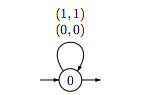
\includegraphics{1}
\newpage
Et pour $L_{+}$ en utilisant des triplets :  \\

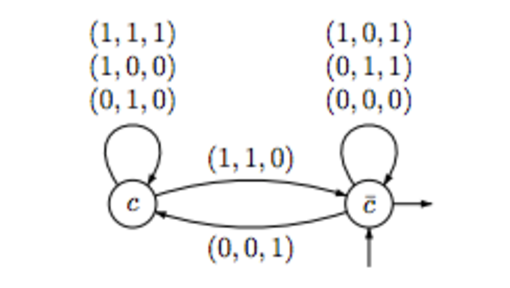
\includegraphics{2}

Cet automate vérifie l'addition "à l'envers". L'état $c$ correspondant à la retenue et l'autre à l'absence de retenue.

\end{solution}

\begin{problem}[Question 3]
En déduire que pour tout $\phi$ formule sans quantificateurs avec $p$ variables libres l'ensemble suivant est rationnel : \\
$$ L_{\phi} = \{ (n_{1}, \, n_{2}, \, \dots , \, n_{p}) \, \, | \, \, \phi(n_{1}, \, n_{2}, \, \dots , \, n_{p}) \text{ vraie} \}$$

\end{problem}

\begin{solution}

On a vu que les composants atomiques de $\phi$ donnent des langages rationnels. On va récupérer $L_{\phi}$ par intersection, union ou complémentation des sous langages correspondant à ces formes atomiques (on peut les étendre à $p$ variables en ignorant les $p-2$ ou $p-3$ composantes qui ne servent à rien). Ça reste rationnel.

\end{solution}

\begin{problem}[Question 4]
Étant donnée une formule $\psi$ sous forme prénexe $\psi = Q_{1}x_{1}Q_{2}x_{2} \, \dots \, Q_{n}x_{n}\hat \psi$, on définit $\psi_k = Q_{k+1}x_{k+1} \, \dots \, Q_{n}x_{n}\hat \psi$.
Montrer par récurrence que les langages suivant sont rationnels :%
$$ X_{k} = \{(x_{1}, x_{2}, \, \dots , \, x_{k}) \, \, | \, \, \psi_k(x_{1}, x_{2}, \, \dots , \, x_{k}) \text{ vraie} \}$$
\end{problem}
\newpage
\begin{solution}
On suppose ici que $\psi$ ne possède pas de variables libres (elle est close). \\
Par définition $\psi_{k}$ possède $k$ variables libres. On procède par récurrence descendante. Par convention : $\psi_{0} = \psi$ et $\psi_{n} = \hat \psi$.
\begin{itemize}
\item $k=n$ : $ X_{n} = \{(x_{1}, x_{2}, \, \dots , \, x_{n}) \, \, | \, \, \hat \psi(x_{1}, x_{2}, \, \dots , \, x_{n}) \text{ vraie} \}$ est rationnel par \textbf{Question 3} puisque $\hat \psi$ est sans quantificateur.
\item \textbf{Hérédité} : Soit $0 \leq k < n $ on suppose $X_{k+1}$ rationnel. \\ On a donc un AFD $\mathcal{A}_{k+1}$ sur l'alphabet $\{0,1\}^{k+1}$ qui reconnait $X_{k+1}$. \\
On va construire $\mathcal{A}_{k}$ sur  $\{0,1\}^{k}$ qui reconnait $X_{k}$.
\\
$ \psi_k = Q_{k+1}x_{k+1} \psi_{k+1}$. Deux cas :

\begin{itemize}
\item $Q_{k+1} = \exists$ : \\ La formule devient : $ \psi_k = \exists x_{k+1} \psi_{k+1}$. Et alors si pour $\mathcal{A}_{k}$ on prend $\mathcal{A}_{k+1}$ où l'on supprime la dernière composante de chaque transition, on trouve un automate non déterministe où l'acceptance d'un mot $(x_{1},\, \dots, \, x_{k})$ revient à l'existence d'un $x_{k+1}$ (formé par un certain choix de la composante qu'on a enlevé sur chaque transition) tel que $\mathcal{A}_{k+1}$ accepte $(x_{1},\, \dots, \, x_{k+1})$. La réciproque est vraie, si $\mathcal{A}_{k+1}$ accepte $(x_{1},\, \dots, \, x_{k+1})$ en prenant le même chemin, $\mathcal{A}_{k}$ accepte $(x_{1},\, \dots, \, x_{k})$.  $\mathcal{A}_{k}$ convient donc et $X_{k}$ est rationnel.
\item $Q_{k+1} = \forall$ : \\ On se ramène au cas précédent par équivalence de $\psi_{k}$ avec $\neg \exists x_{k+1} \neg \psi_{k+1}$. On conclut par stabilité des langages rationnels par passage au complémentaire.
\end{itemize}
\end{itemize}
D'où le résultat.
\end{solution}

\begin{problem}[Question 5]
Conclure en considérant $X_{0}$.
\end{problem}

\begin{solution}
On a $\psi_{0} =  \psi$. 
\begin{itemize}
\item Si $\psi = \forall x_{1} \psi_{1}(x_{1})$ on doit vérifier que $X_{1} = \mathcal{L}(\mathcal{A}_{1}) = \{0,1\}^{*}$
\item Si $\psi = \exists x_{1} \psi_{1}(x_{1})$ on doit vérifier que $X_{1} = \mathcal{L}(\mathcal{A}_{1}) \neq \emptyset$
\end{itemize}
Ces deux problèmes sont décidables. \\ \\
On peut aussi conclure avec $\mathcal{A}_{0}$ associé à $X_{0}$ : 
$\mathcal{A}_{0}$ est un graphe orienté. \\
Par la construction des $\mathcal{A}_{k}$ il suffit désormais de tester l'accessibilité d'un état final à partir d'un état initial (on conclut en fonction de $Q_{1}$) ce qui est décidable. \\
D'où le résultat.
\end{solution}
\newpage
\begin{problem}[Question 6]
Faites tourner l'algorithme sur les formules : 

\begin{align*}
\psi_{0}(x) \equiv \, \, & \exists  y, \, \exists z , \, x = y+z \land z = y + y \\
\psi_{1} \equiv \, \, & \forall x , \, \psi_{0}(x)
\end{align*}

\end{problem}

\begin{solution}
La première formule est équivalente à l'équation $x \equiv 0 \, \, mod \, \, 3$, on veut donc montrer que $\psi_{1}$ est fausse. \\
Pour $x = y + z \land z = y + y$ on propose l'automate suivant : \\
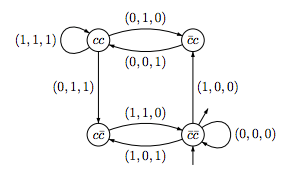
\includegraphics{3}
\\
On utilise l'agorithme pour trouver l'automate associé à $\psi_{0}$, après déterminisation on trouve : 
\\
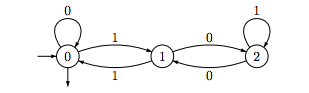
\includegraphics{4}
\\
On se rend compte que la formule est fausse puisque $1$ n'est pas dans le langage de cet automate (voir première conclusion \textbf{Question 5}). \\
D'où le résultat.
\end{solution}

\newpage

\problemlist{Exercice 2}
On définit le problème $Term$ (resp. $Conf$) de la manière suivante : étant donné un système
de réécriture de termes $\mathcal{R}$, est ce que $\mathcal{R}$ est terminant (resp. confluent). \\

\begin{problem}[Question 1]
Expliquer comment coder des mots dans un système de termes.
\end{problem}
\begin{solution}
On suppose que les mots sont codés dans $\{0,1\}^{*}$. \\
On peut par exemple se donner deux symboles unaires $0(x)$ et $1(x)$ ainsi qu'un symbole
constant $\circ$.  Par exemple on code $01001$ par $0(1(0(0(0(1(\circ))))))$.\\
De manière générale on code $u = u_{0} \dots u_{n}$ par $u_{0}( \dots u_{n}( \circ) \dots )$.\\
On notera directement $u(x)$.
\end{solution}


\begin{problem}[Question 2]
Exhiber une réduction de PCP vers $Term$ avec une signature contenant un seul symbole
de fonction ternaire $f$ (en plus de ce qui est nécessaire pour simuler des mots).
\end{problem}
\begin{solution}
Soit une instance $<\alpha_{i}, \beta_{i}>$ de PCP. On va montrer qu'on peut lui associer un système de réécriture qui ne termine pas si et seulement si cette instance possède une solution. \\
On prend la signature $\sum = \{\circ,\, 0(x),\, 1(x),\, g(x,y,z)\}$. On définit les règles :

\begin{align*}
r_{i} : & \quad g(\alpha_{i}(x), \, \beta_{i}(y), \, z) \quad \to \quad g(x,y,z) \\
r_{\circ,0} : & \quad g(\circ, \, \circ, \, 0(x)) \quad \to \quad g(0(x),0(x),0(x)) \\
r_{\circ,1} : & \quad g(\circ, \, \circ, \, 1(x)) \quad \to \quad g(1(x),1(x),1(x))
\end{align*}
\noindent
Grâce à ces règles on va pouvoir créer des cycles : $g(\circ, \circ, u(\circ)) \to g(u(\circ), u(\circ), u(\circ))$. \\

\begin{itemize}
\item Supposons que l'instance est une solution : $\alpha_{i_{1}} \dots \alpha_{i_{m}} \equiv \beta_{i_{1}} \dots \beta_{i_{m}}$, on pose $u = \alpha_{i_{1}} \dots \alpha_{i_{m}}$. Alors en utilisant les règles on va dépiler successivement les deux premiers arguments de $g$ et lorsque $\circ$ est atteint on retrouve la situation initiale. On a bien : 

$$ g(u(\circ),u(\circ),u(\circ)) =  g(\alpha_{i_{1}} \dots \alpha_{i_{m}}(\circ),\beta_{i_{1}} \dots \beta_{i_{m}}(\circ),u(\circ)) \to g(\circ,\circ,u(\circ)) \to g(u(\circ),u(\circ),u(\circ)) $$
Cette réduction est cyclique, le système ne termine pas. \\

\item On suppose que l'instance n'a pas de solution. On veut montrer que $\mathcal{R}$ termine. Ceci par induction sur les termes on montre que tout terme se réduit en un nombre fini d'étapes en une forme normale.

\begin{itemize}
\item \textbf{Cas} $x$ une variable : déjà en forme normale.
\item \textbf{Cas} $\circ$ : idem
\item \textbf{Cas} $0(t)$ : on ne peut appliquer aucune règles, donc par hypothèse d'induction sur $t$ c'est bon.
\item \textbf{Cas} $1(t)$ : idem
\item \textbf{Cas} $t = g(t_{1},t_{2},t_{3})$ : supposons que $t$ possède une suite de réduction infinie. Les règles $r_{i}$ épuisent les deux premières composantes on se retrouve donc nécessairement dans une situation du type $r_{\circ,0}$ ou $r_{\circ,1}$ à un moment de la chaîne de réduction. On a donc un schéma du type :

$$ g(t_{1}, t_{2}, t_{3}) \to^{*} g(\circ, \circ, t_{4}) \to g(t_{4}, t_{4}, t_{4})$$

La séquence est infinie avec le même argument : 

$$ g(t_{4}, t_{4}, t_{4}) \to^{*} g(\circ, \circ, t_{5}) \to g(t_{5}, t_{5}, t_{5}) $$

\end{itemize}

\end{itemize}

\end{solution}


\end{document}




